\documentclass{article}
\usepackage{graphicx}
\usepackage{amsmath}
\usepackage{listings}
\lstset{
language=Python,
frame=single, 
breaklines=true,
columns=fullflexible
}
%Enumering lower case roman numerals
%\renewcommand{\theenumi}{\roman{enumi}}   
%\renewcommand{\labelenumi}{\theenumi)}


\begin{document}

\title{Filter Design}

\author{EE23BTECH11009 - AROSHISH PRADHAN*}

\maketitle
%-------------------------------------------------------------------------------
\section{Introduction}
We are supposed to design the equivalent FIR and IIR filter realizations for a band-pass filter with pass band: $9.4$ kHz and $10.6$ kHz.

\section{Filter Specifications}
The sampling rate for the filter has been specified as $F_s =  48$ kHz.	

\subsection{The Digital Filter}

\begin{enumerate}
\item {\em Tolerances:}  The pass-band ($\delta_1$) and stop-band ($\delta_2$) tolerances are given to
be equal, so we let $\delta_1 = \delta_2 = \delta = 0.15$.

\item {\em Pass-band:}  The pass-band of the filter is calculated as follows: 
\begin{align*}
    j = (r - 11000) \, \text{mod} \, \sigma
\end{align*}
where, 
\begin{align*}
    r &= \text{Roll Number}\\
    &= 11009\\
    \sigma &= \text{Sum of digits of roll number}\\
    &= 11\\
    \implies j &= 9
\end{align*}
The pass band is then given by:
\begin{align*}
    4 + 0.6(j)\,  &\text{to} \, 4 + 0.6( j + 2)\\ 
    \implies 9.4 \text{kHz} \, &\text{to} \, 10.6\text{kHz} 
\end{align*}
Hence, the un-normalized discrete time filter
pass-band frequencies are:
\begin{align*}
    F_{p1} &= 10.6\, \text{kHz}\\
    F_{p2} &= 9.4\, \text{kHz}
\end{align*}
If the un-normalized  discrete-time (natural) frequency is F, the corresponding normalized digital filter (angular) frequency is given by $\omega = 2\pi
\left(\frac{F}{F_s}\right)$. Therefore,
\begin{align*}
\omega_{p1} &= 2\pi\frac{F_{p1}}{F_s}  = 0.441\pi\\ \omega_{p2} &= 2\pi\frac{F_{p2}}{F_s}  = 0.391\pi 
\end{align*}
The centre frequency is then given by  $\omega_c = \frac{\omega_{p1} + \omega_{p2}}{2} = 0.416\pi$.  

\item {\em Stop-band:}  The {\em transition band} for band-pass filters is $\Delta F = 0.3$ kHz on either side of the pass-band.
Hence, the un-normalized {\em stop-band} frequencies are:
\begin{align*}
F_{s1} &= 10.6 + 0.3 = 10.9\, \text{kHz}\\
F_{s2} &= 9.4 - 0.3 = 9.1\, \text{kHz}
\end{align*}
The corresponding normalized frequencies are:
\begin{align*}
    \omega_{s1} = 0.454 \pi\\
    \omega_{s2} =  0.379 \pi
\end{align*}
The above parameters are summarized in the table below:
\begin{table}[!h]
    \centering
    \begin{tabular}{|c|c|c|}
    \hline
       \textbf{Symbol}  & \textbf{Value} &  \textbf{Description}\\
    \hline
       $V_{in}$  &  &  Input Voltage\\
    \hline
        $V_{out}$ & & Output Voltage\\
    \hline
        $f$ & $1000Hz$ & Input Wave Frequency\\
    \hline
        $T$ & $\dfrac{1}{f} = 10^{-3} s$ & Input Wave Time Period\\
    \hline
        \multirow{4}{*}{$R$} & (a) $0.5k\Omega$ & \multirow{4}{*}{Resistance}\\
        \cline{2-2}
        & (b) $5k\Omega$ &\\
        \cline{2-2}
        & (c) $0.5k\Omega$ &\\
        \cline{2-2}
        & (d) $5k\Omega$ &\\
    \hline
        \multirow{4}{*}{$C$} & (a) $0.1\mu F$ & \multirow{4}{*}{Capacitance}\\
        \cline{2-2}
        & (b) $1\mu F$ &\\
        \cline{2-2}
        & (c) $0.1\mu F$ &\\
        \cline{2-2}
        & (d) $1\mu F$ &\\
    \hline
        $\tau$ & $RC$ & Time Constant\\
    \hline
    \end{tabular}
    \caption{Given Parameters}
    \label{tab:1_gate.23.ph.37}
\end{table}

\end{enumerate}

\subsection{The Analog filter}
In the bilinear transform, the analog filter frequency ($\Omega$) is related to the corresponding digital filter frequency ($\omega$) as $\Omega = \tan \frac{\omega}{2}$.  Using this relation, we obtain the analog pass-band and stop-band frequencies as:
\begin{align*}
\Omega_{p1} &= \tan\left(\frac{\omega_{p_1}}{2}\right) = 0.8298\\ 
\Omega_{p2} &= \tan\left(\frac{\omega_{p_2}}{2}\right) = 0.7051\\
\Omega_{s1} &= \tan\left(\frac{\omega_{s_1}}{2}\right) = 0.8649\\
\Omega_{s2} &= \tan\left(\frac{\omega_{s_2}}{2}\right) =  0.6772
\end{align*}
respectively.

\section{The IIR Filter Design}
{\em Filter Type:}  We are supposed to design filters whose stop-band is monotonic and pass-band equiripple.  
Hence, we use the {\em Chebyschev approximation} to design our band-pass IIR filter.

\subsection{The Analog Filter}
\begin{enumerate}

\item {\em Low Pass Filter Specifications:}  If $H_{a, BP}(j\Omega)$ be the desired analog band
pass filter,  with the specifications provided in Section 2.2, and $H_{a,LP}(j\Omega_L)$ 
be the equivalent low pass filter, then
\begin{equation}
\label{transition}
\Omega_L = \frac{\Omega^2 - \Omega_0^2}{B\Omega}
\end{equation}

%\begin{equation}
%H_{a, BP}(j\Omega) =  H_{a,LP}(j\Omega_L) \vert_{ \Omega_L = 
%\frac{\Omega^2 - \Omega_0^2}{B\Omega}},
%\end{equation}
where 
\begin{align*}
\Omega_0 &= \sqrt{\Omega_{p1}\Omega_{p2}} = 0.7649\\
B &= \Omega_{p1} - \Omega_{p2} = 0.1247\\
	\implies \Omega_{L_{p_1}} &= \frac{\Omega_{p_1}^2 - \Omega_{p_1}\Omega_{p_2}}{(\Omega_{p_1} - \Omega_{p_2})\Omega_{p_1}} = 1
\end{align*}
The low pass filter has
the pass-band edge at $\Omega_{Lp} = 1$ and stop-band edges at 
\begin{align*}
    \Omega_{L_{s_1}} &= \frac{\Omega_{s_1}^2 - \Omega_0^2}{B\Omega_{s_1}} =  1.5111\\
    \Omega_{L_{s_2}} &= \frac{\Omega_{s_2}^2 - \Omega_0^2}{B\Omega_{s_2}} = -1.4976
\end{align*}
We choose the stop-band edge of the analog low pass filter as $\Omega_{Ls} = \mbox{min}(\vert \Omega_{Ls_1}\vert,\vert \Omega_{Ls_2}\vert) = 1.4976$.

\item {\em The Low Pass Chebyschev Filter Parameters:}  The magnitude squared of the Chebyschev low pass filter is given by 
\begin{equation}
\label{lpfirst}
\vert H_{a,LP}(j\Omega_L)\vert^2 = \frac{1}{1 + \epsilon^2c_N^2\left(\frac{\Omega_L}{\Omega_{L_p}}\right)}
\end{equation}
where $c_N(x)$ is the Chebyshev Polynomial of the first kind of order $N$, given by:

\begin{align*}
    c_N(x) = \begin{cases}
        \cos(N\cos^{-1}(x)) & \text{if } \lvert x \rvert \leq 1\\
        \operatorname{cosh}(N\cosh^{-1}(x)) & \text{if } x \geq 1\\
    \end{cases}
\end{align*}
where N and $\epsilon$ are design parameters.  Since $\Omega_{Lp} = 1$, (\ref{lpfirst}) may be rewritten as
\begin{equation}
\label{lpsecond}
\vert H_{a,LP}(j\Omega_L)\vert^2 = \frac{1}{1 + \epsilon^2c_N^2(\Omega_L)}
\end{equation}
Also, the design paramters have the following constraints
\begin{eqnarray}
\label{lpdesign}
\frac{\sqrt{D_2}}{c_N(\Omega_{Ls})} \leq \epsilon \leq \sqrt{D_1}, \nonumber \\
N \geq \left\lceil \frac{\cosh^{-1}\sqrt{D_2/D_1}}{\cosh^{-1}\Omega_{Ls}} \right\rceil,
\end{eqnarray}
where 
\begin{align*}
    D_1 &= \frac{1}{(1 - \delta)^2}-1 = 0.384\\
    D_2 &= \frac{1}{\delta^2} - 1 = 43.444
\end{align*}
After substituting $\delta = 0.15$ and $\Omega_{L_s} = 1.4976$, 
we obtain $N \geq 4$ and $0.2897 \leq \epsilon \leq 0.6197$.  In Fig. \ref{fig:low_pass}, we plot $\vert H(j\Omega)\vert$ for a range of values of $\epsilon$, for $N = 4$.  We find that for larger values of $\epsilon$, $|H(j\Omega)|$ decreases in the transition band.  We choose $\epsilon = 0.4$  for our IIR filter design.
\begin{lstlisting}[caption = {Code for Figure 1}]
wget https://github.com/aroshishp/EE1205/blob/main/Filter_Design/codes/low_pass.py
\end{lstlisting}
\begin{figure}[!h]
    \centering
    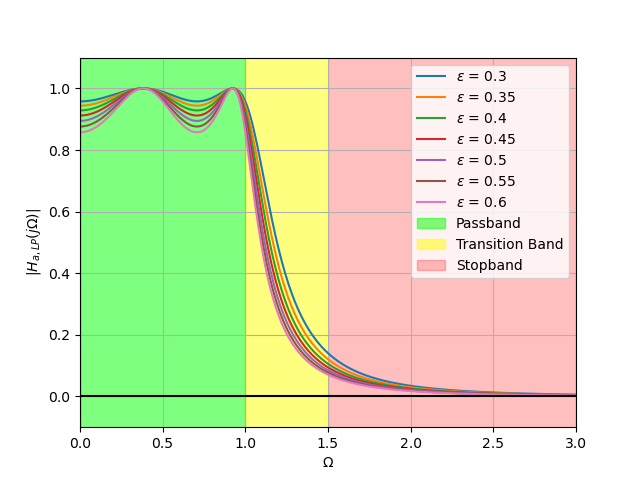
\includegraphics[width = \columnwidth]{figs/low_pass.png}
    \caption{Analog Low-Pass Frequency Response for $0.3 \leq \epsilon \leq 0.6$}
    \label{fig:low_pass}
\end{figure}
\newpage
\item {\em The Low Pass Chebyshev Filter:} Thus, we obtain
\begin{equation}
\label{lpsqfinal}
\vert H_{a,LP}(j\Omega_L)\vert^2 = \frac{1}{1 + 0.16c_4^2(\Omega_L)}
\end{equation}
where,
\begin{equation}
c_4(x) = 8x^4 - 8x^2 + 1.	
\end{equation}
The poles of the frequency response in (\ref{lpsqfinal}) lying on the left half of the Argand Plane are in general obtained as
\begin{align}
    s_k = r_1\cos(\phi_k)+ jr_2\sin( \phi_k) \label{eq: 7}
\end{align}
where
\begin{eqnarray}
\label{lppoles}
\phi_k = \frac{\pi}{2} + \frac{(2k+1)\pi}{2N}, k = 0, 1, \dots, N-1 \nonumber \\
r_1 = \frac{\beta^2 - 1}{2\beta}, r_2 = \frac{\beta^2 + 1}{2\beta}, \beta = \left[ \frac{\sqrt{1 + \epsilon^2} + 1}{\epsilon}\right]^{\frac{1}{N}}
\end{eqnarray}
Values of $s_k$ using \eqref{eq: 7} are given in the table below:
\begin{table}[!h]
    \centering
    \begin{tabular}{|c|c|}
    \hline
       $s_k$  &  \textbf{Value}\\
    \hline
       $s_0$  & $-0.162 + 1.003j$\\
    \hline
       $s_1$  & $-0.391 + 0.415j$\\
    \hline
       $s_2$  & $-0.391 - 0.415j$\\
    \hline
       $s_3$  & $-0.162 - 1.003j$\\
    \hline
    \end{tabular}
    \caption{Poles on left half of complex plane}
    \label{tab:2}
\end{table}


Note that the poles of frequency response in \eqref{lpsqfinal} are calculated through the below code separately and plotted in Figure \ref{fig:2}.\\
\begin{table}[!h]
    \centering
    \begin{tabular}{|c|c|}
    \hline
       $s_k$  &  \textbf{Value}\\
    \hline
       $s_0$  & $-0.162 + 1.003j$\\
    \hline
       $s_1$  & $-0.391 + 0.415j$\\
    \hline
       $s_2$  & $-0.391 - 0.415j$\\
    \hline
       $s_3$  & $-0.162 - 1.003j$\\
    \hline
       $s_4$  & $0.162 + 1.003j$\\
    \hline
       $s_5$  & $0.391 + 0.415j$\\
    \hline
       $s_6$  & $0.391 - 0.415j$\\
    \hline
       $s_7$  & $0.162 - 1.003j$\\
    \hline
    \end{tabular}
    \caption{Poles of frequency response in \eqref{lpsqfinal}}
    \label{tab:3}
\end{table}

\begin{lstlisting}[caption = {Code for Figure 2}]
wget https://github.com/aroshishp/EE1205/blob/main/Filter_Design/codes/poleplot.py
\end{lstlisting}

\begin{figure}[!h]
    \centering
    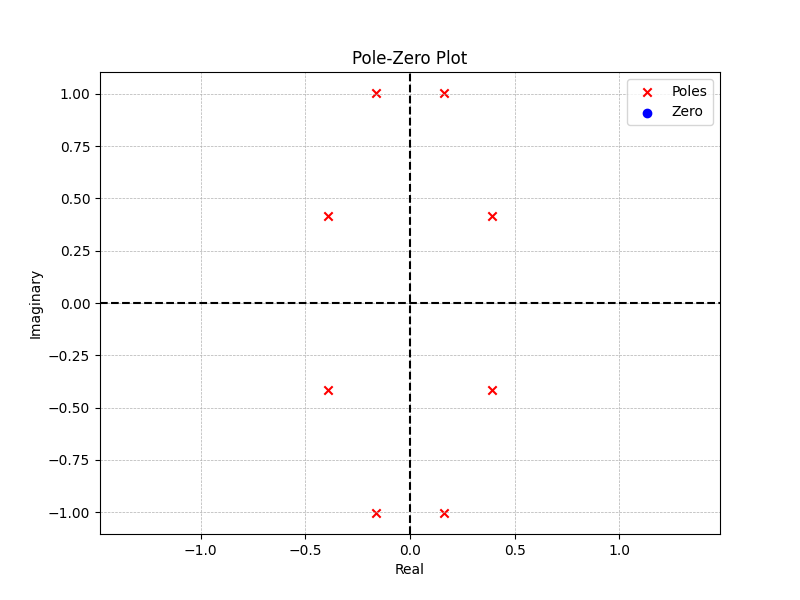
\includegraphics[width = \columnwidth]{figs/pole_zero.png}
    \caption{Pole-Zero Plot of frequency response of \eqref{lpsqfinal}}
    \label{fig:2}
\end{figure}
\newpage
Thus, for even $N$, the low-pass stable Chebyshev filter, with a gain $G_{LP}$ has the form
\begin{align}
\label{poleleft}
H_{a,LP}(s_L) &= \frac{G_{LP}}{\prod_{k = 1}^{\frac{N}{2}-1}(s_L^2 - 2r_1\cos\phi_ks_L + r_1^2\cos^2\phi_k + r_2^2 \sin^2\phi_k)}\\
&= \frac{G_{LP}}{(s - s_0)(s - s_1)(s - s_2)(s - s_3)}
\end{align}
Substituting $N = 4$, $\epsilon = 0.4$ and $H_{a,LP}(j) = \frac{1}{\sqrt{1+\epsilon^2}}$, from (\ref{lppoles}) and (\ref{poleleft}), we obtain 
\begin{equation}
\label{lpfinal}
H_{a,LP}(s_L) = \frac{0.3125}{s_L^4 + 1.1068s_L^3 + 1.6125s_L^2+0.9140s_L + 0.3366}
\end{equation}
In Figure 3 we plot $|H(j\Omega)|$ using (\ref{lpsqfinal}) and (\ref{lpfinal}), thereby verifying that our low-pass Chebyschev filter design meets the specifications.
\begin{lstlisting}[caption = {Code for Figure 3}]
wget https://github.com/aroshishp/EE1205/blob/main/Filter_Design/codes/verification.py
\end{lstlisting}
\begin{figure}[!h]
    \centering
    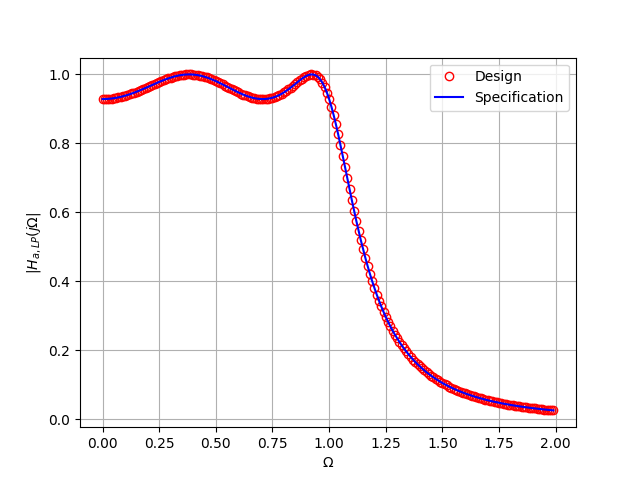
\includegraphics[width = \columnwidth]{figs/verification.png}
    \caption{Plot of Frequency Response obtained from specifications in \eqref{lpsqfinal}} and design in \eqref{lpfinal}
    \label{fig:3}
\end{figure}
\item {\em The Band Pass Chebyschev Filter:}  The analog band-pass filter is obtained from (\ref{lpfinal}) as follows. From \eqref{transition}:
\begin{align}
    \Omega_L &= \frac{\Omega^2 - \Omega_0^2}{B\Omega}\\
    \implies j\Omega_L &= \frac{\Omega_0^2 - \Omega^2}{Bj\Omega}\\
    &= \frac{\Omega_0^2 + (j\Omega)^2}{Bj\Omega}\\
    \implies s_L &= \frac{s^2 + \Omega_0^2}{Bs}
\end{align}
Hence, 
\begin{equation}
H_{a,BP}(s) = G_{BP}H_{a,LP}(s_L)\vert_{s_L = \frac{s^2 + \Omega_0^2}{Bs}},
\end{equation}
where $G_{BP}$ is the gain of the band-pass filter. The below code evaluates $G_{BP}$ and finds the coefficients of $H_{a, BP}$. We get $G_{BP} = 1.077$ by evaluating gain  
such that $H_{a,BP}(j\Omega_{p1}) = 1$.
{\tiny
\begin{equation}
\label{bpfinal}
H_{a,BP}(s) = \frac{7.55642\times 10^{-5}s^4}{s^8+0.138015s^7+2.36536s^6+0.244019s^5+2.08328s^4+0.142769s^3+0.809685s^2+0.0276411s+0.117176}
\end{equation}
}
In Figure \ref{fig:4}, we plot $\vert H_{a,BP}(j\Omega)\vert$ as a function of $\Omega$ for both positive as
well as negative frequencies.  We find that the pass-band and stop-band frequencies in the figure
match well with those obtained analytically through the bilinear transformation.
\begin{lstlisting}[caption = {Code for Figure 4}]
wget https://github.com/aroshishp/EE1205/blob/main/Filter_Design/codes/Hbp.py
\end{lstlisting}
\end{enumerate}
\begin{figure}[!h]
    \centering
    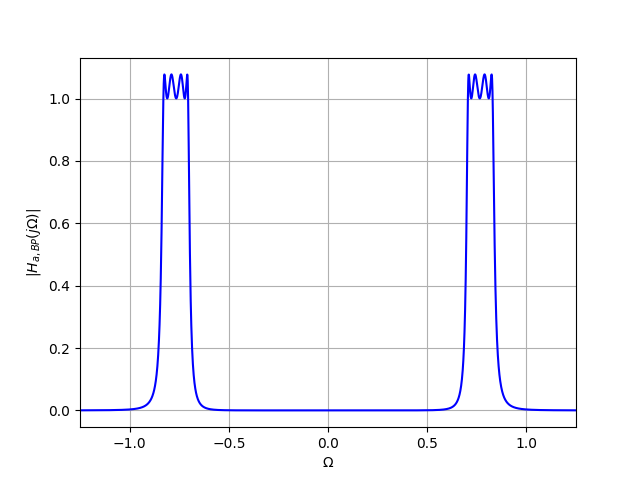
\includegraphics[width= \columnwidth]{figs/Hbp.png}
    \caption{Analog Band-Pass Frequency Response from \eqref{bpfinal}}
    \label{fig:4}
\end{figure}



\subsection{The Digital Filter}
From the bilinear transformation, we obtain the digital band-pass filter from the corresponding analog filter as
\begin{eqnarray}
\label{analdig}
H_{d,BP}(z) = GH_{a,BP}(s)\vert_{s = \frac{1-z^{-1}}{1 + z^{-1}}}
\end{eqnarray}
where $G$ is the gain of the digital filter.  From (\ref{bpfinal}) and (\ref{analdig}), we obtain

\begin{eqnarray}
H_{d,BP}(z) = G \frac{N(z)}{D(z)}
\end{eqnarray}
All coefficients and $G$ are calculated from the below code.
\begin{lstlisting}[caption = {Code for G, N(z), D(z)}]
wget https://github.com/aroshishp/EE1205/blob/main/Filter_Design/codes/substitutor.py
\end{lstlisting}

We get:
\begin{align}
    G &= 7.55642 \times 10^{-5}\\
    N(z) &=  1 - 4 z^{-2} + 6 z^{-4} - 4z^{-6} + z^{-8}\\
    D(z) &= 5.8230569z^{-8} - 12.4205486z^{-7} + 34.1023786z^{-6} - 42.2777094z^{-5}\nonumber \\
  &+ 58.95155z^{-4} - 44.1531786z^{-3} + 37.1935974z^{-2} - 14.1500354z^{-1}\nonumber\\
  &+ 6.9279451
\end{align}

The plot of $|H_{d,BP}(z)|$ with respect to the normalized angular freqency (normalizing factor $\pi$) is available in Figure \ref{fig:5}.  Again we
find that the pass-band and stop-band frequencies meet the specifications well enough.
\begin{lstlisting}[caption = {Code for Figure 5}]
wget https://github.com/aroshishp/EE1205/blob/main/Filter_Design/codes/Hdbp.py
\end{lstlisting}
\begin{figure}[!h]
    \centering
    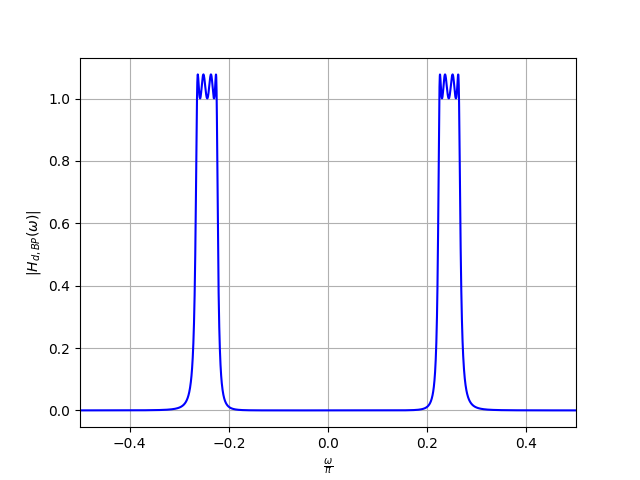
\includegraphics[width = 0.9\columnwidth]{figs/H_dbp.png}
    \caption{The magnitude response of the band-pass digital filter}
    \label{fig:5}
\end{figure}

\section{The FIR Filter}
We design the FIR filter by first obtaining the (non-causal) low-pass equivalent using the Kaiser window
and then
converting it to a causal band-pass filter.

\subsection{The Equivalent Low-Pass Filter}
The low-pass filter has a pass-band frequency $\omega_l$ and transition band $\Delta \omega = 2\pi \frac{\Delta F}{F_s} = 0.0125\pi$.
The stop-band tolerance is $\delta$.
\begin{enumerate}
\item  The {\em pass-band frequency $\omega_l$}  is defined as:
\begin{align}
    \omega_l = \frac{\omega_{p1} - \omega_{p2}}{2} = 0.025\pi
\end{align}
Substituting the values of $\omega_{p1}$ and $\omega_{p2}$ from section 2.1, we obtain $\omega_l = 0.025\pi$.

\item {\em The impulse response $h_{lp}(n)$} of the desired low-pass filter with cutoff frequency $\omega_l$
is given by
\begin{eqnarray}
\label{firlpdef}
h_l(n) = \frac{\sin(n\omega_l)}{n\pi}w(n),
\end{eqnarray}
where $w(n)$ is the Kaiser window obtained from the design specifications.
\end{enumerate}

\subsection{The Kaiser Window}
The Kaiser window is defined as
\begin{eqnarray}
\label{kaiser}
w(n) &=& \frac{I_0\left[ \beta N \sqrt{1 - \left(\frac{n}{N}\right)^2} \right]}{I_0(\beta N)},
\indent -N \leq n \leq N, \indent \beta > 0 \nonumber \\
&=& 0 \hspace{5cm} \mbox{otherwise,}
\end{eqnarray}
where $I_0(x)$ is the modified Bessel function of the first kind of order zero in $x$ and $\beta$
and $N$ are the window shaping factors.  In the following,
we find $\beta$ and $N$ using the design parameters in section 2.1.

\begin{enumerate}
\item  N is chosen according to
\begin{equation}
N \geq \frac{A-8}{4.57\Delta \omega},
\end{equation}
where $A = -20\log_{10}\delta$.  Substituting the appropriate values from the design specifications, we obtain
$A = 16.4782$ and $N \geq 48$.

\item  $\beta$ is chosen according to
\begin{eqnarray}
\label{kaisercond}
\beta N = \left\{ \begin{array}{ll} 0.1102(A-8.7) & A > 50 \\
0.5849(A-21)^{0.4}+ 0.07886(A-21) & 21 \leq A \leq 50 \\
0 & A < 21\end{array} \right.
\end{eqnarray}
In our design, we have $A = 16.4782 < 21$.  Hence, from (\ref{kaisercond}) we obtain $\beta = 0$.  

\item We choose $N = 100$, to ensure the desired low pass filter response.  Substituting in (\ref{kaiser})
gives us the rectangular window
\begin{eqnarray}
\label{rect}
w(n) &=& 1, \indent -100 \leq n \leq 100 \nonumber \\
&=& 0 \hspace{6mm} \mbox{otherwise}
\end{eqnarray}
\end{enumerate}

From (\ref{firlpdef}) and (\ref{rect}), we obtain the desired low-pass filter impulse response
\begin{eqnarray}
\label{firlpfinal}
h_{lp}(n) &=& \frac{\sin(\frac{n\pi}{40})}{n\pi} \indent -100 \leq n \leq 100 \nonumber \\
&=& 0, \hspace{2cm} \mbox{otherwise}
\end{eqnarray}
\begin{lstlisting}[caption = {Code for Figure 6 and 7}]
wget https://github.com/aroshishp/EE1205/blob/main/Filter_Design/codes/fir_hH.py
\end{lstlisting}
\begin{figure}[!h]
    \centering
    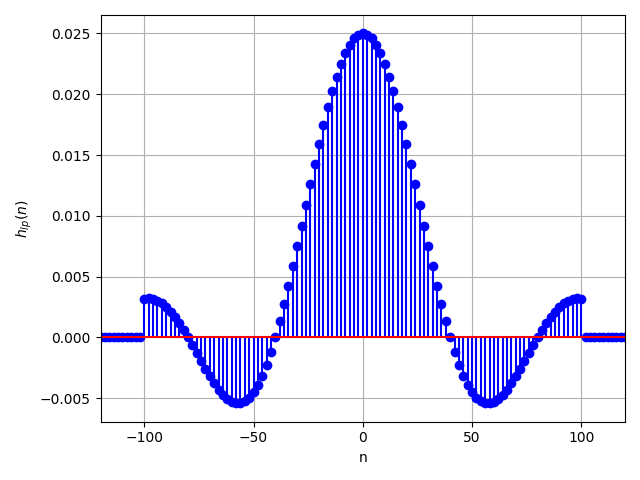
\includegraphics[width = \columnwidth]{figs/fir_hlp.png}
    \caption{Plot of FIR Low-Pass Filter Impulse Response}
    \label{fig:6}
\end{figure}

The magnitude of the Frequency Response of low-pass filter is plotted in Figure \ref{fig:7}.

\begin{figure}[!h]
    \centering
    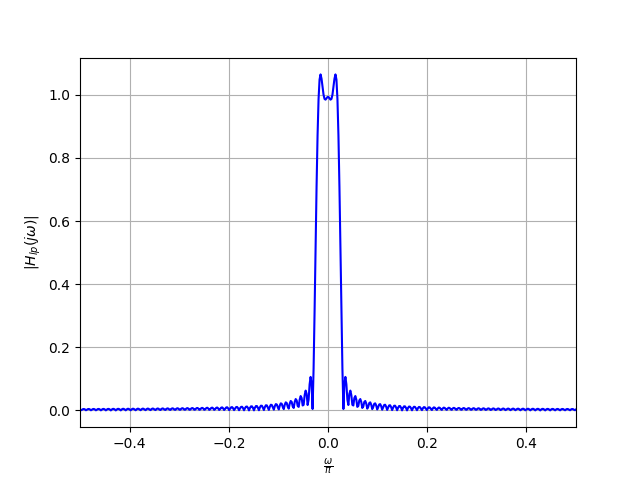
\includegraphics[width = \columnwidth]{figs/firHLP.png}
    \caption{Plot of FIR Low-Pass Filter Frequency Response}
    \label{fig:7}
\end{figure}
\subsection{The FIR Band-pass Filter}
The centre of the pass-band of the desired band-pass filter was found to be $\omega_c = 0.416\pi$ in Section
2.1.  The impulse response of the desired band-pass filter is obtained from the impulse response of the
corresponding low-pass filter as
\begin{eqnarray}
h_{bp}(n) = 2h_{lp}(n)cos(n\omega_c)
\end{eqnarray}
Thus, from (\ref{firlpfinal}), we obtain (plotted in Figure \ref{fig:8})
\begin{eqnarray}
\label{firbpfinal}
h_{bp}(n) &=& \frac{2\sin(\frac{n\pi}{40}) \cos(0.416n\pi)}{n\pi} \indent -100 \leq n \leq 100 \nonumber \\
&=& 0, \hspace{4cm} \mbox{otherwise}
\end{eqnarray}
\begin{lstlisting}[caption = {Code for Figure 8 and 9}]
wget https://github.com/aroshishp/EE1205/blob/main/Filter_Design/codes/fir_bp.py
\end{lstlisting}

The magnitude response of the FIR band-pass filter designed to meet the given specifications is plotted in Figure \ref{fig:9}.
\begin{figure}[!h]
    \centering
    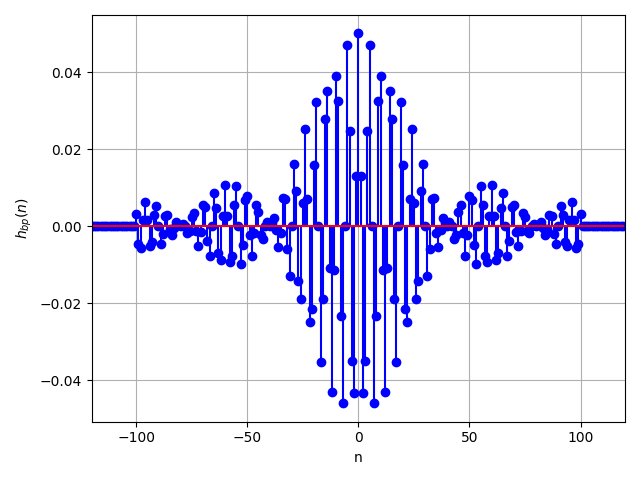
\includegraphics[width = 0.95\columnwidth]{figs/fir_hbp.png}
    \caption{Plot of FIR Band-Pass Filter Impulse Response}
    \label{fig:8}
\end{figure}
\begin{figure}[!h]
    \centering
    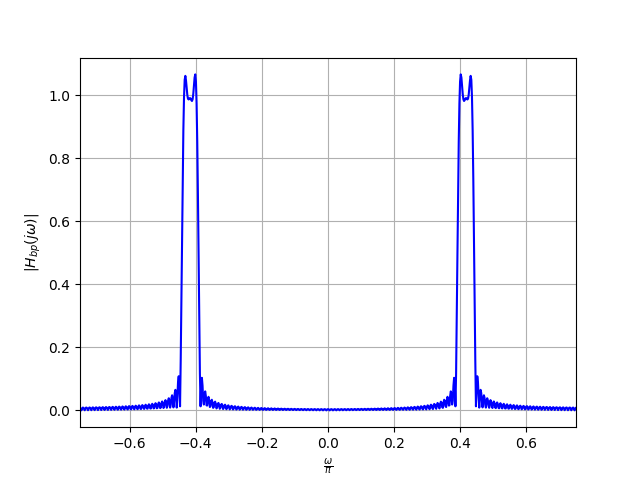
\includegraphics[width = 0.95\columnwidth]{figs/firHbp.png}
    \caption{Plot of FIR Band-Pass Filter Frequency Response}
    \label{fig:9}
\end{figure}
\end{document}}
